%%%%%%%%%%%%%%%%%%%%%%%%%%%%%%%%%%%%%%%%%
% The Legrand Orange Book
% LaTeX Template
% Version 3.1 (February 18, 2022)
%
% This template originates from:
% https://www.LaTeXTemplates.com
%
% Authors:
% Vel (vel@latextemplates.com)
% Mathias Legrand (legrand.mathias@gmail.com)
%
% License:
% CC BY-NC-SA 4.0 (https://creativecommons.org/licenses/by-nc-sa/4.0/)
%
% Compiling this template:
% This template uses biber for its bibliography and makeindex for its index.
% When you first open the template, compile it from the command line with the 
% commands below to make sure your LaTeX distribution is configured correctly:
%
% 1) pdflatex main
% 2) makeindex main.idx -s indexstyle.ist
% 3) biber main
% 4) pdflatex main x 2
%
% After this, when you wish to update the bibliography/index use the appropriate
% command above and make sure to compile with pdflatex several times 
% afterwards to propagate your changes to the document.
%
%%%%%%%%%%%%%%%%%%%%%%%%%%%%%%%%%%%%%%%%%

%----------------------------------------------------------------------------------------
%	PACKAGES AND OTHER DOCUMENT CONFIGURATIONS
%----------------------------------------------------------------------------------------

\documentclass[
	11pt, % Default font size, select one of 10pt, 11pt or 12pt
	fleqn, % Left align equations
	a4paper, % Paper size, use either 'a4paper' for A4 size or 'letterpaper' for US letter size
	%oneside, % Uncomment for oneside mode, this doesn't start new chapters and parts on odd pages (adding an empty page if required), this mode is more suitable if the book is to be read on a screen instead of printed
]{LegrandOrangeBook}

% Book information for PDF metadata, remove/comment this block if not required 


\addbibresource{sample.bib} % Bibliography file

\definecolor{ocre}{RGB}{243, 102, 25} % Define the color used for highlighting throughout the book

\chapterimage{orange2.jpg} % Chapter heading image
\chapterspaceabove{6.5cm} % Default whitespace from the top of the page to the chapter title on chapter pages
\chapterspacebelow{6.75cm} % Default amount of vertical whitespace from the top margin to the start of the text on chapter pages

%----------------------------------------------------------------------------------------
\usepackage{csquotes}
\begin{document}




%----------------------------------------------------------------------------------------
%	TITLE PAGE
%----------------------------------------------------------------------------------------

\titlepage % Output the title page
	{
\includegraphics[width=\paperwidth]{Images/background.pdf}} % Code to output the background image, which should be the same dimensions as the paper to fill the page entirely; leave empty for no background image
	{ % Title(s) and author(s)
		\centering\sffamily % Font styling
		{\Huge\bfseries TS CPRP 1 \\ Sciences de l'ingénieur\par} % Book title
		\vspace{16pt} % Vertical whitespace
		{\LARGE Séquence 2 : Représenter les pièces dans une MOCN\par} % Subtitle
		\vspace{24pt} % Vertical whitespace
		{\huge\bfseries \par} % Author name
	}









%----------------------------------------------------------------------------------------
%	SECTIONING EXAMPLES CHAPTER
%----------------------------------------------------------------------------------------


\part{Les MOCN dans le noir}

%----------------------------------------------------------------------------------------
%	MATHEMATICS EXAMPLES CHAPTER
%----------------------------------------------------------------------------------------

\chapter{Allumer le feu}

\section{Les ingrédients pour usiner}


En BTS CPRP, nous nous intéresseront au machines ayant des outils qui sont commandés numériquement par un programme informatique. Quand on achète une MOCN, elle dispose déjà d'un programme interne. Nous devons cependant le modifier pour qu'il réponde à notre besoin. Comme en informatique, chaque programme à un but précis. Nous auront en principe un programme à entrer dans la machine par pièce que nous souhaitons usiner. Pour programmer, vous connaissez sûrement déjà certain langage de programmation : on peut citer le C++, HTML, CSS, Python, Arduino, etc. Cependant les programmes utilisés pour l'usinage sont assez spécifiques et changent moins que dans d'autres domaines\footnote{Les langages de programmation pour le code ou les sites internet évoluent sans cesse, pour un codeur informatique, le choix du langage est très large par rapport à notre domaine.}. À l'origine, le langage de programmation était le \textbf{G-code}\footnote{, Développé par l'EIA (Electronic Industries Alliance) au début des années 1960.}, et finalement remplacé par l'\textbf{ISO}\footnote{Remplacé en février 1980 sous la référence RS274D.} mais certain constructeur peuvent avoir d'autre langage propre à la marque du constructeur.


\begin{figure}[H] % Use [H] to suppress floating and place the figure/table exactly where it is specified in the text
	\centering % Horizontally center the figure on the page
	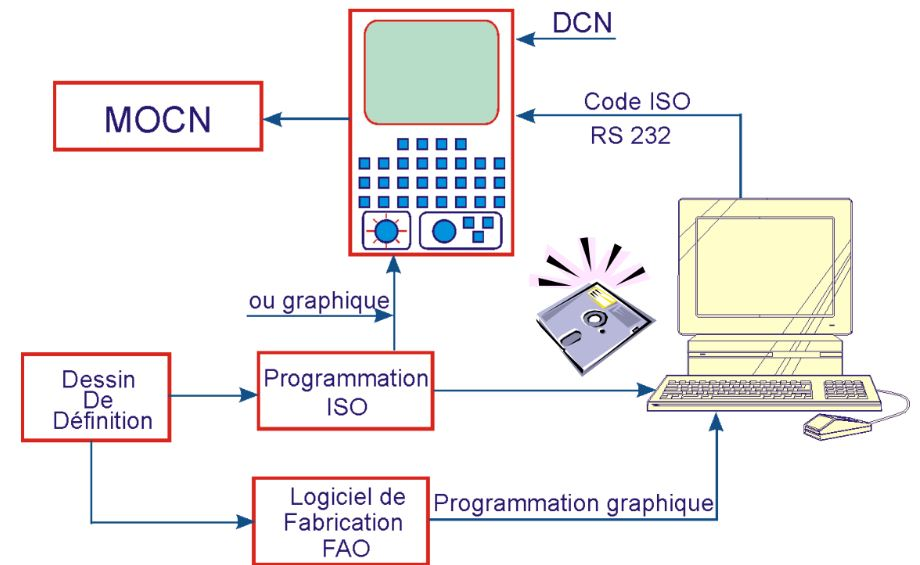
\includegraphics[width=0.7\textwidth]{Images/iso.JPG} % Include the figure image
	\caption{Chargement d'un programme dans une MOCN. Université des Sciences et de la Technologie d'Oran Mohamed-Boudiaf USTOMB}
	\label{iso3} % Unique label used for referencing the figure in-text
\end{figure}



Les machines ne sont pas comme nous, sans aucune perception de leur environnements elles sont dans le noir. Et nous leur demandons d'usiner avec une grande précision. Si on veut la longueur maximum d'une pièce de 20,001 mm mais que la pièce sortie mesure 20,002 : elle sera à jeter... Tout cela avec des vitesses très lente ou très rapide (0,001 m/min à 130 m/min). \\



Alors dans tout ça, de quoi avons-nous besoin ? \\

\begin{theorem}
\begin{itemize}
    \item Un objet de départ dont on va enlever la matière : \textit{\textbf{Le brut de matière}} ;
    \item Des éléments pour enlever la matière : \textit{\textbf{Les outils}} ;
    \item De la force ! pour trancher, percer, tronçonner, fournit par : \textit{\textbf{Des moteurs}} ; 
    \item Oui mais si j'essaye de couper une feuille de papier avec des ciseaux, sans la tenir dans l'autre main c'est difficile, il faut donc que le \textit{Brut} soit solidement "attaché" : La \textit{\textbf{MIP}} et le \textit{\textbf{MAP}}\footnote{La MIP (MIse en Position) et le MAP (MAintient en Position) seront abordés plus tard dans l'année dans différents cours, mais surtout en industrialisation.}  ;
    \item  Pour faire la forme que l'on veut : \textit{\textbf{Une trajectoire}} ;
\end{itemize}
\end{theorem}

Dans la suite nous allons nous intéresser au dernier point. \textit{Repérer les éléments dans l'espace.} 

Pour usiner, nous avons besoin de plusieurs informations à chaque instant $t$, la position de l'outil qui usine, sa vitesse, son accélération, sa trajectoire. Ces informations doivent être calculées puis programmées dans la machine. Nous allons voir dans ce chapitre comment construire l'information : repérer les objets dans les MOCN.


\section{Outil mathématique pour futur.s.es l'ingénieur : Vous}

Un \textit{repère} sera présent pour \textbf{toutes} les études, analyses, interrogations que vous verrez. On ne peut pas faire sans. Sinon on ne serait pas capable de décrire ce que l'on voit sous forme mathématique et donc impossible à programmer dans une machine. Un \textit{repère} est constitué de deux choses : Une $\mathcal{B}ase$ et une Origine. On l'écrit comme suit : $\mathcal{R}(0, \Vec{x}, \Vec{y}, \Vec{z})$.\\
On lit la phrase suivante : Voici $\mathcal{R}$, un repère constitué d'une origine $O$ et d'une $\mathcal{B}ase$ de vecteurs $\Vec{x}$, $\Vec{y}$, $\Vec{z}$. \\
La $\mathcal{B}ase$, c'est le tableau Excel infini, où sont présents tous les vecteur (en deux ou trois dimensions), mais ils ne peuvent pas être égaux. Par exemple, $\Vec{a}=\ \begin{Bmatrix} 1\\ 3 \end{Bmatrix} $ et $\Vec{b}=\ \begin{Bmatrix} 1\\ 3 \end{Bmatrix}$  ne peuvent pas être élus au rang de $\mathcal{B}ase$ car ils sont égaux. En revanche, dans la bibliothèque infinie il y a les vecteurs $\Vec{i}=\ \begin{Bmatrix} -1\\ 3 \\ 0 \end{Bmatrix} $ et $\Vec{j}=\ \begin{Bmatrix} -1\\ 0 \\ 3\end{Bmatrix}$ qui peuvent être choisi pour faire une base. \\



\begin{figure}[H] % Use [H] to suppress floating and place the figure/table exactly where it is specified in the text
	\centering % Horizontally center the figure on the page
	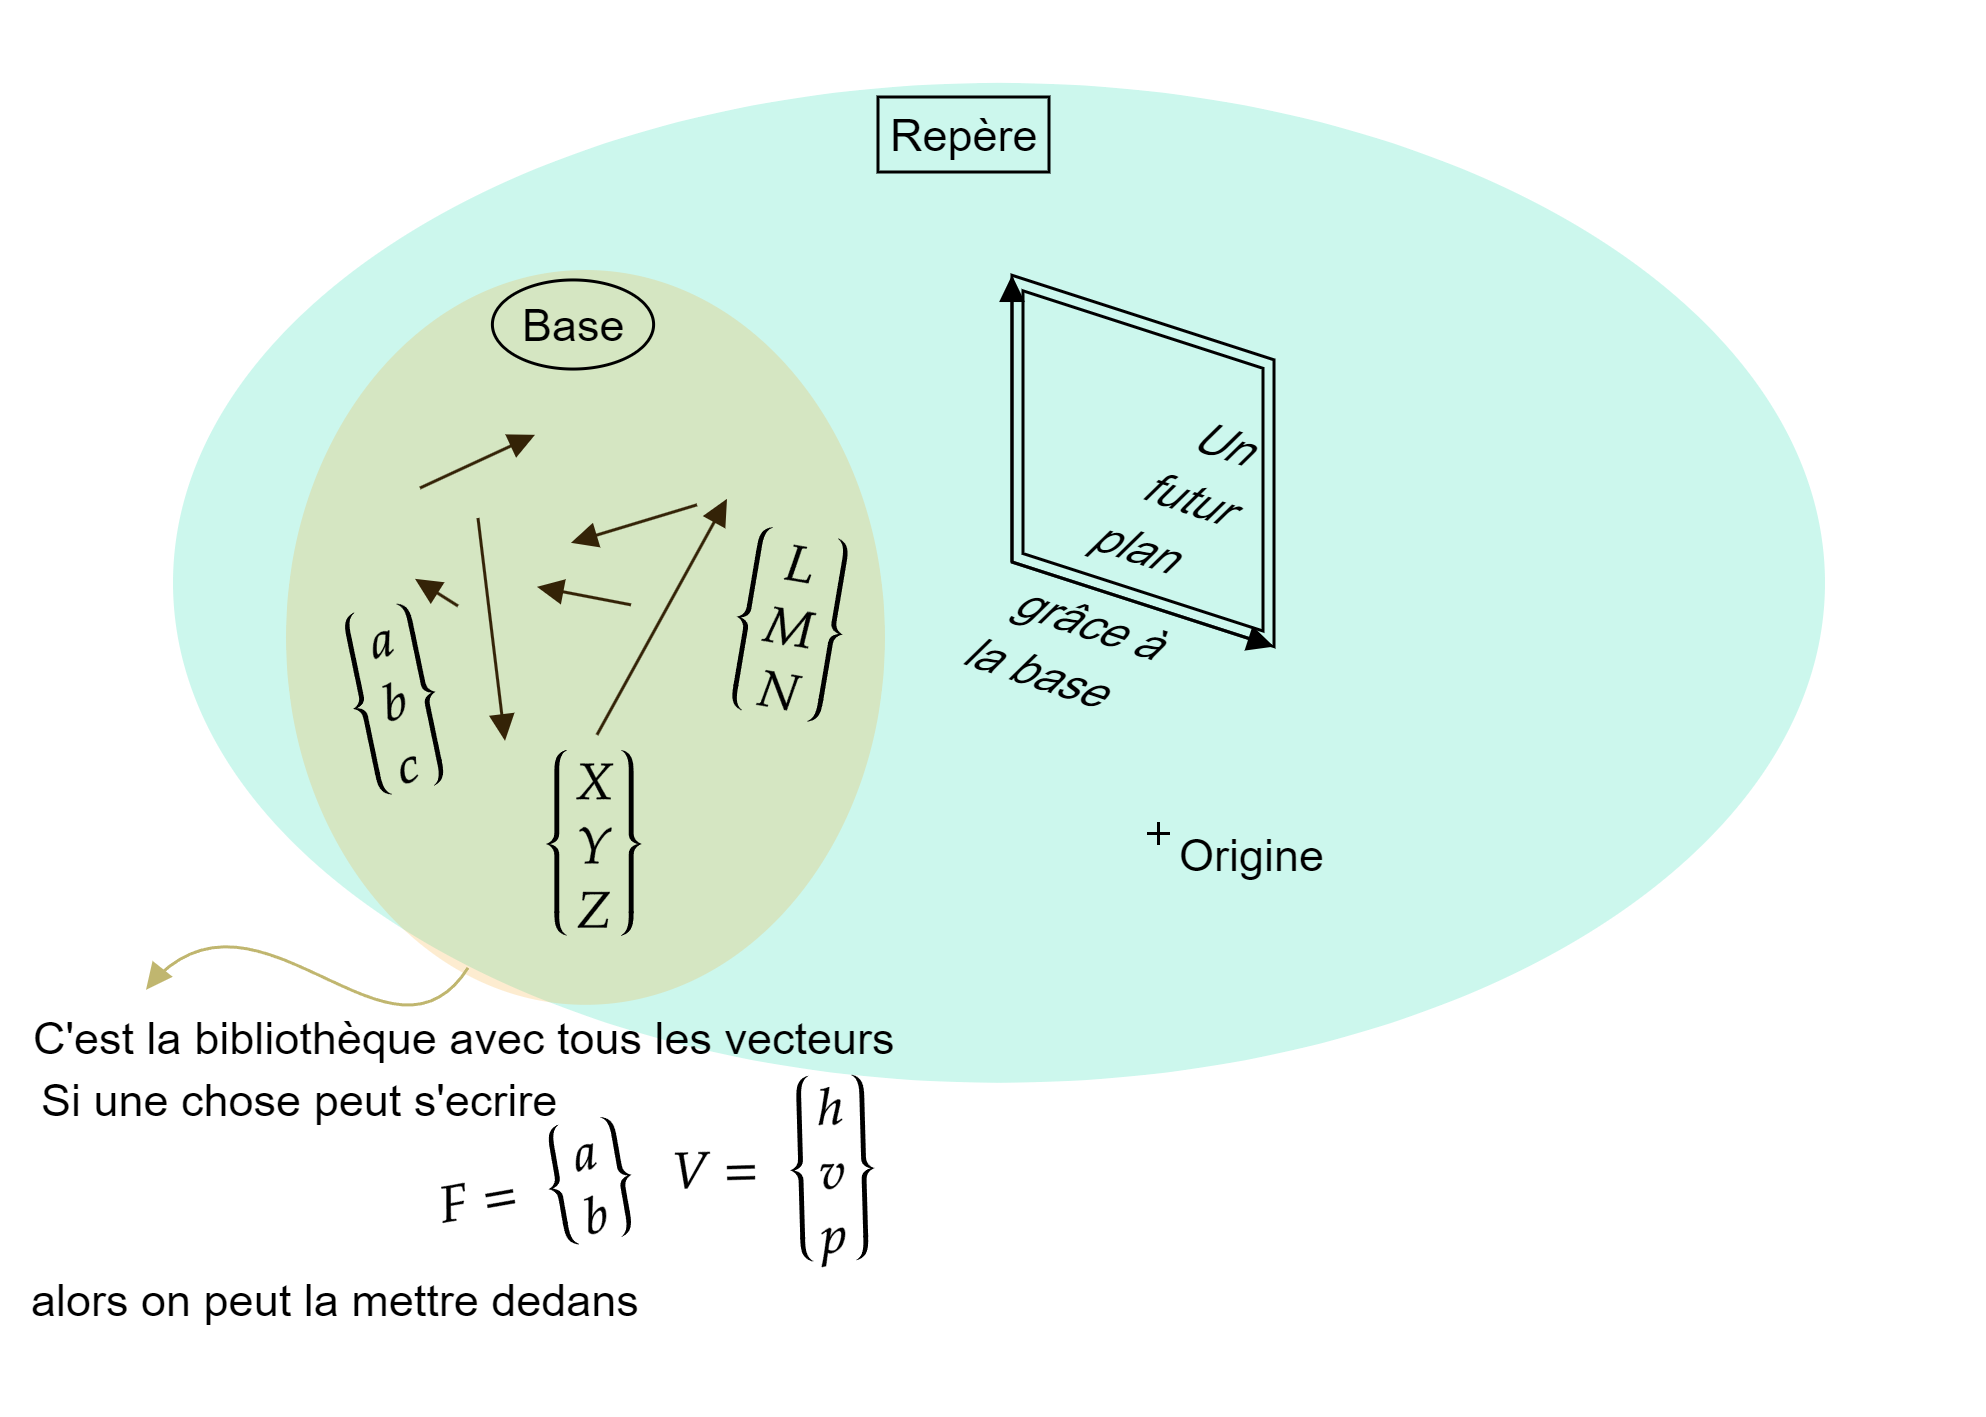
\includegraphics[width=1.1\textwidth]{Images/vect1.png} % Include the figure image
	\caption{Éléments pour construire un repère}
	\label{vect1} % Unique label used for referencing the figure in-text
\end{figure}


Un repère $\mathcal{R}$ est la donnée d’un point d'origine $\mathcal{O}$ et d’une base $\mathcal{B}$, permettant de repérer tous points de
l’espace par rapport à $\mathcal{O}$ (l'origine du repère). On décide que $\mathcal{O}$ est notre origine, on choisi deux vecteurs dans notre bibliothèque (sauf s'il sont égaux), on prend l'origine des deux vecteurs et on le colle sur notre point $\mathcal{O}$. Voilà, le repère est fait. \\

\begin{remark}
    En pratique, nous n'avons pas besoin de dire si un vecteur ou un repère est en 2 ou 3 dimensions. Un vecteur en 2 dimensions possède 2 données $\Vec{i}=\ \begin{Bmatrix} a\\ b \end{Bmatrix} $, il en possédera trois, pour la dimension trois : $\Vec{i}=\ \begin{Bmatrix} a\\ b \\ c \end{Bmatrix} $. De même, un repère en deux dimensions s'écriera $\mathcal{R}(0, \Vec{x}, \Vec{y})$, tandis-qu'un repère à trois dimensions s'écriera $\mathcal{R}(0, \Vec{x}, \Vec{y}, \Vec{z})$.    
\end{remark}

\begin{figure}[H] % Use [H] to suppress floating and place the figure/table exactly where it is specified in the text
	\centering % Horizontally center the figure on the page
	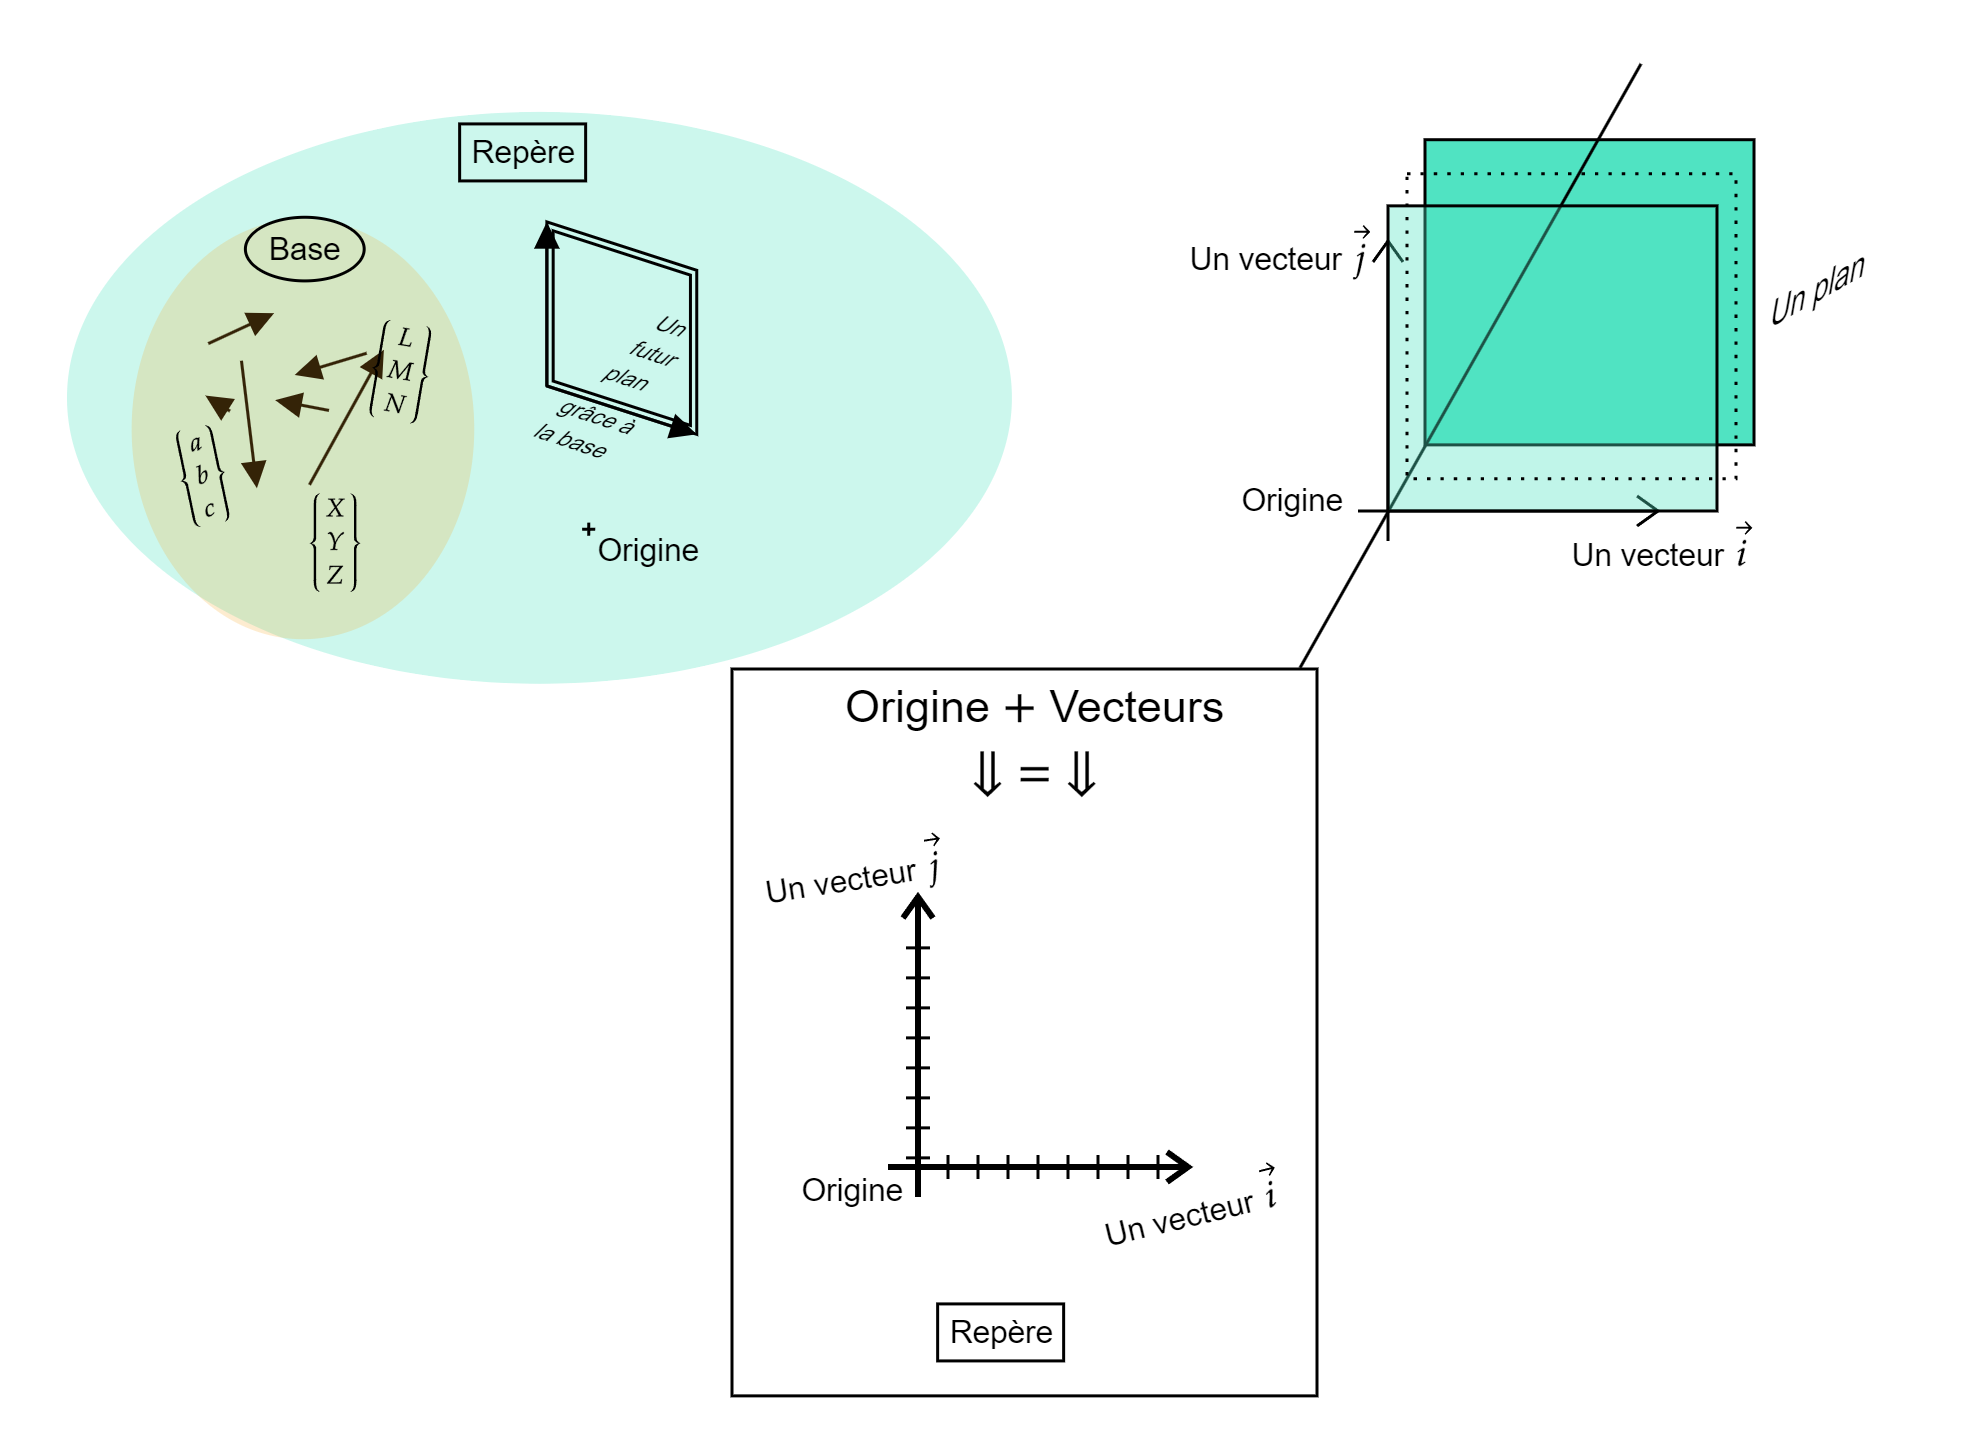
\includegraphics[width=1.1\textwidth]{Images/vect2.png} % Include the figure image
	\caption{Symbolisation d'un repère. Une fois une base (deux vecteurs) et une origine ($\mathcal{O}$) choisies, les deux vecteurs mis bout à bout forme un plan, et $\mathcal{O}$ nous sert à connaître n'importe quel point par rapport à lui.}
	\label{vect2} % Unique label used for referencing the figure in-text
\end{figure}

Maintenant que nous avons vu le cas général, nous allons voir les cas que vous croiserez en pratique. Que ce soit en théorie ou en pratique, en contrôle ou à l'examen, il y a quelque situation à connaître pour ne pas être surpris.e.

\section{Ortho-normé-direct}

Cette expression, vous la verrez beaucoup. Nous avons vu comment construire un repère, mais ceux qui seront utilisés pour les exercices ou en examens seront pour la plupart du temps construit pour être le plus simple possible. Nous allons détailler les repères principaux, qui sont orthogonaux, normés et directs.

\begin{figure}[H] % Use [H] to suppress floating and place the figure/table exactly where it is specified in the text
	\centering % Horizontally center the figure on the page
	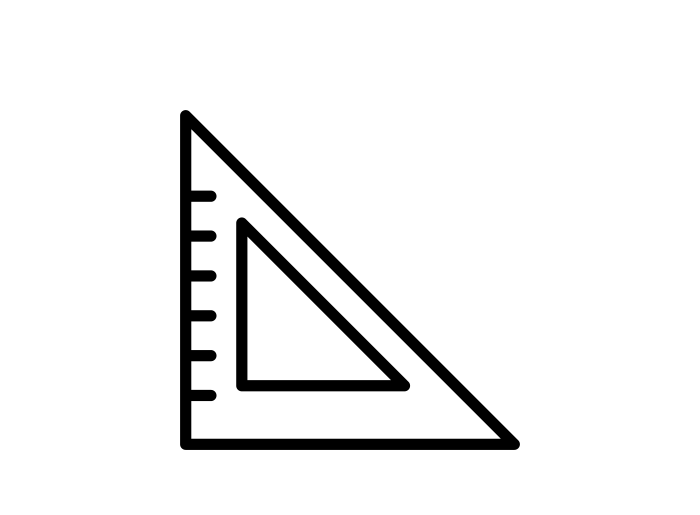
\includegraphics[width=0.25\textwidth]{Images/tri.png} % Include the figure image
    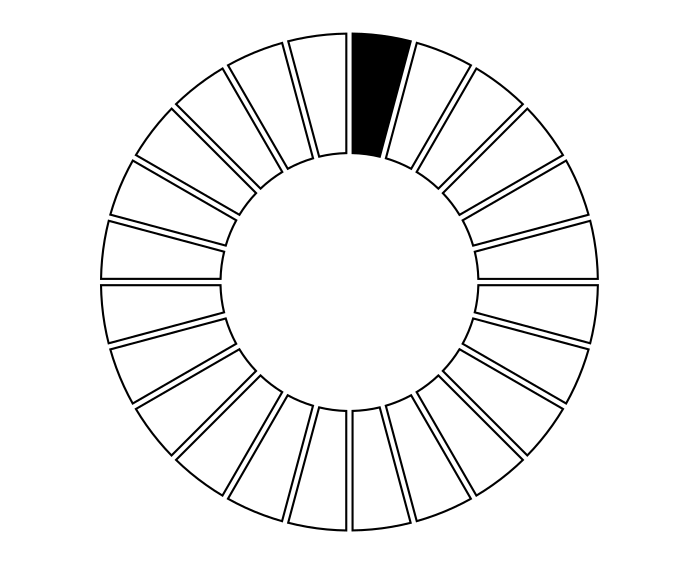
\includegraphics[width=0.2\textwidth]{Images/one.png} % Include the figure image
    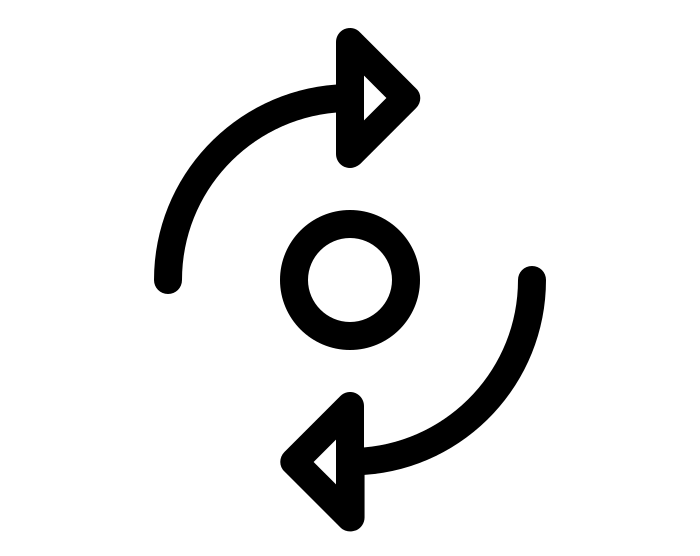
\includegraphics[width=0.2\textwidth]{Images/rot.png} % Include the figure image

\end{figure}




\subsection{Orthogonalité}
Les vecteurs que nous prenons dans notre bibliothèque (la $\mathcal{B}ase$) ne seront en général pas pris au hasard. On s'arrangera avoir deux vecteurs simplement perpendiculaires. 

\begin{figure}[H] % Use [H] to suppress floating and place the figure/table exactly where it is specified in the text
	\centering % Horizontally center the figure on the page
	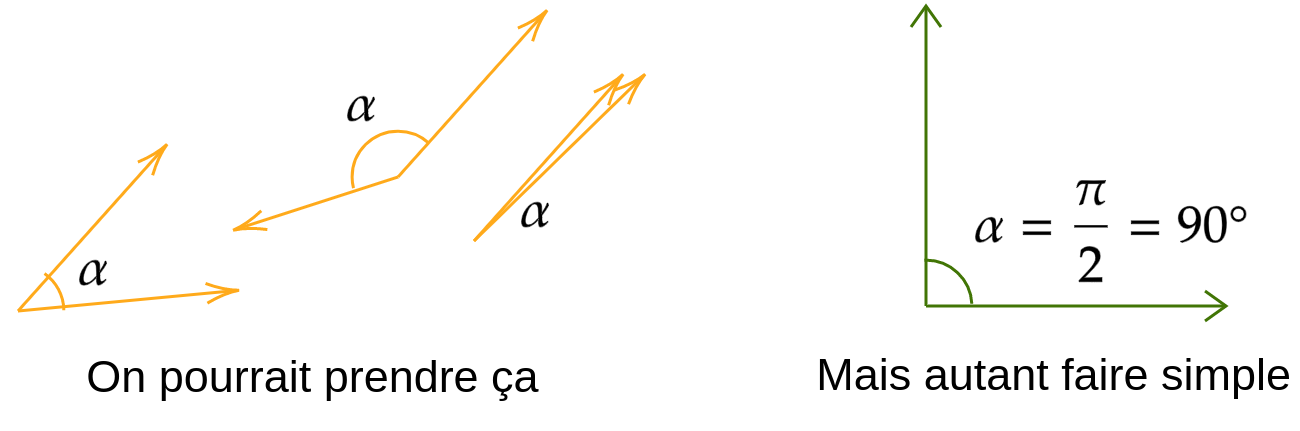
\includegraphics[width=0.8\textwidth]{Images/ortho1.png} % Include the figure image
	\label{ortho1} % Unique label used for referencing the figure in-text
\end{figure}

L'avantage est qu'une rotation d'un demi tour ($180^{\circ}$) sera égal à $\pi$ ce qui simplifie grandement les calculs.







\subsection{Normé}

Une autre simplification est la normalisation des vecteurs utilisés pour construire une base. 
\begin{figure}[H] % Use [H] to suppress floating and place the figure/table exactly where it is specified in the text
	\centering % Horizontally center the figure on the page
	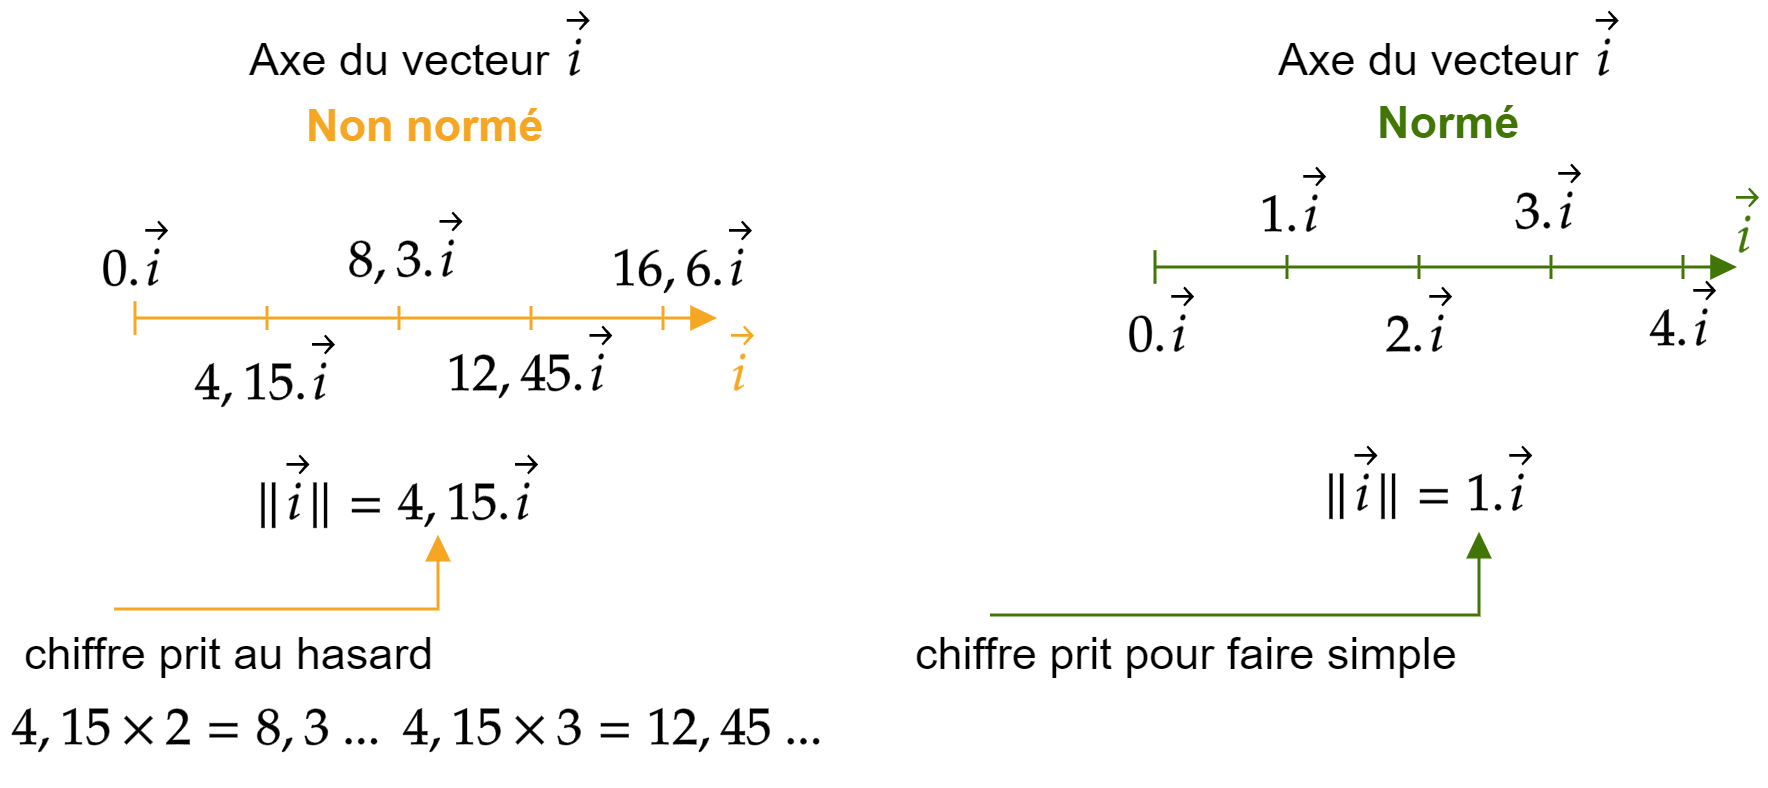
\includegraphics[width=1\textwidth]{Images/norme2.png} % Include the figure image
	\caption{Construction d'une base avec des vecteurs à norme unitaire.}
	\label{norme2} % Unique label used for referencing the figure in-text
\end{figure}

La distance entre chaque trait d'un repère dit normé est de \textit{une} unité. L'aspect plus scientifique des \textit{vecteurs unitaires} sera détaillé dans le chapitre [\ref{Vecteurs}] dédié.

\begin{theorem}
    Un vecteur qui possède une norme de une unité est appelé \textbf{vecteur unitaire}. On écrit : $ \Vert \Vec{u} \Vert = 1\ $
\end{theorem}



\subsection{Direct}

En choisissant un repère dit \textit{direct}, on choisira une fois pour toute, le sens \textbf{positif} de rotation entre les axes. En grande majorité, on prendra le sens \textbf{anti-horaire}, donc \textbf{trigonométrique}. Cela simplifiera les calculs, notamment pour toutes les formules de trigonométrie. De plus, il est important d'avoir un outil commun, par exemple pour décrire la rotation d'une vis dans son logement les calculs négatifs ou positifs peuvent décrire un vissage ou dévissage et une erreur de compréhension doit être évitée.

\begin{figure}[H] % Use [H] to suppress floating and place the figure/table exactly where it is specified in the text
	\centering % Horizontally center the figure on the page
	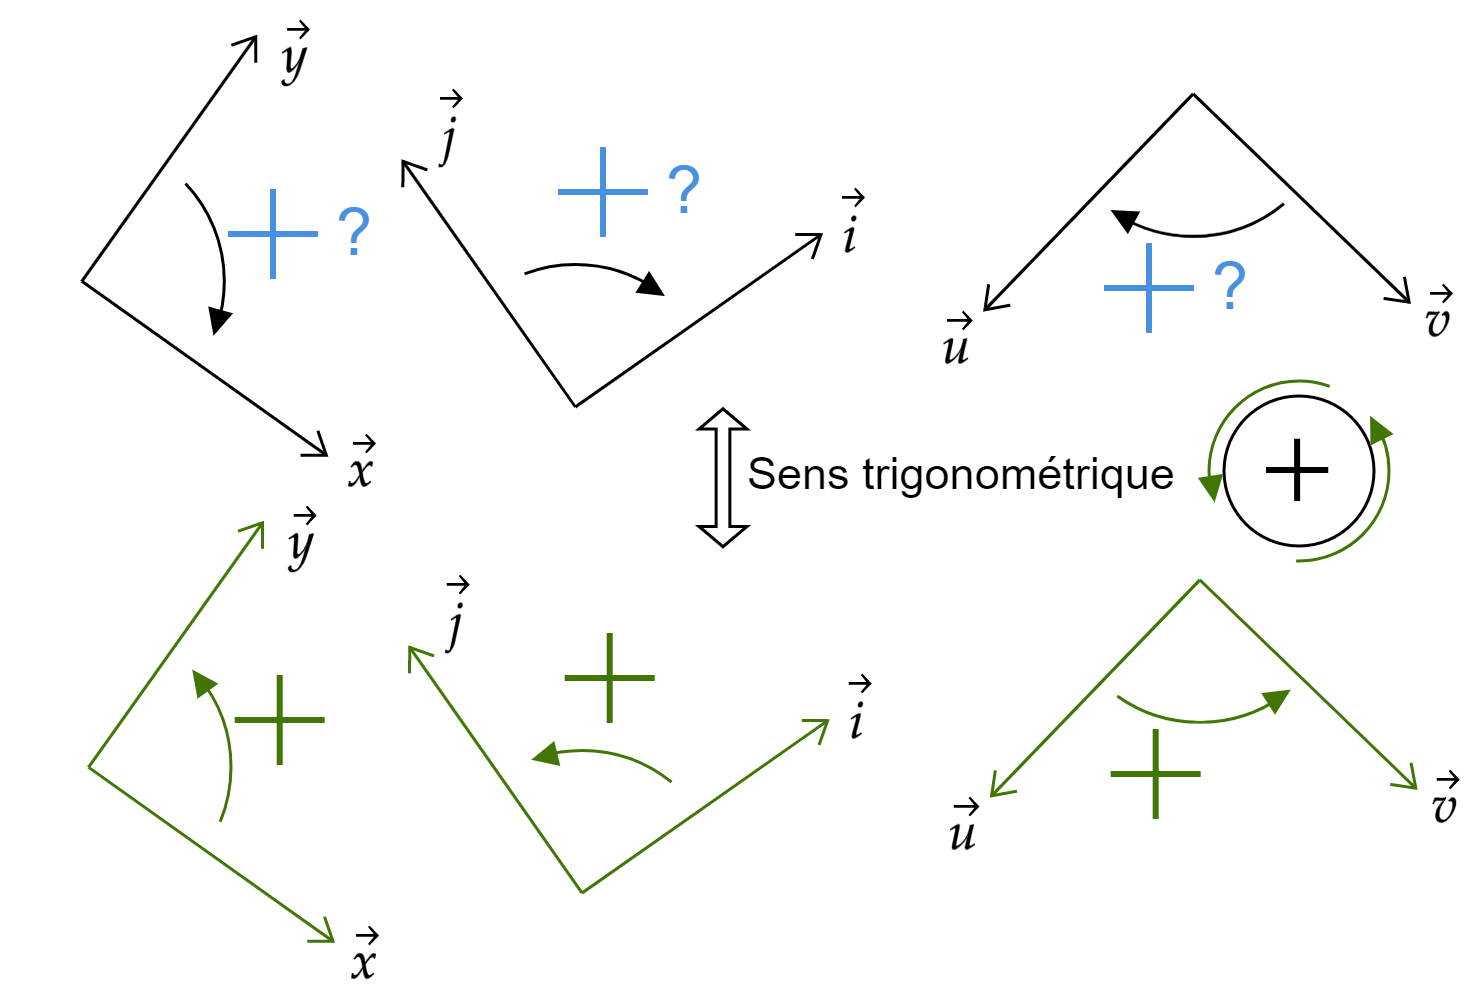
\includegraphics[width=0.8\textwidth]{Images/direct1.png} % Include the figure image
	\caption{Construction d'une base suivant le sens trigonométrique.}
	\label{direct1} % Unique label used for referencing the figure in-text
\end{figure}



\begin{theorem}
Au final, on aura donc un repère qui en général, se composera de deux vecteurs non égaux et unitaires, qui seront mis bout à bout et perpendiculaires. L'endroit de leur rencontre sera le point d'origine du repère. Et le sens sera positif quand on suivras le sens trigonométrique.
\end{theorem}

\begin{figure}[H] % Use [H] to suppress floating and place the figure/table exactly where it is specified in the text
	\centering % Horizontally center the figure on the page
	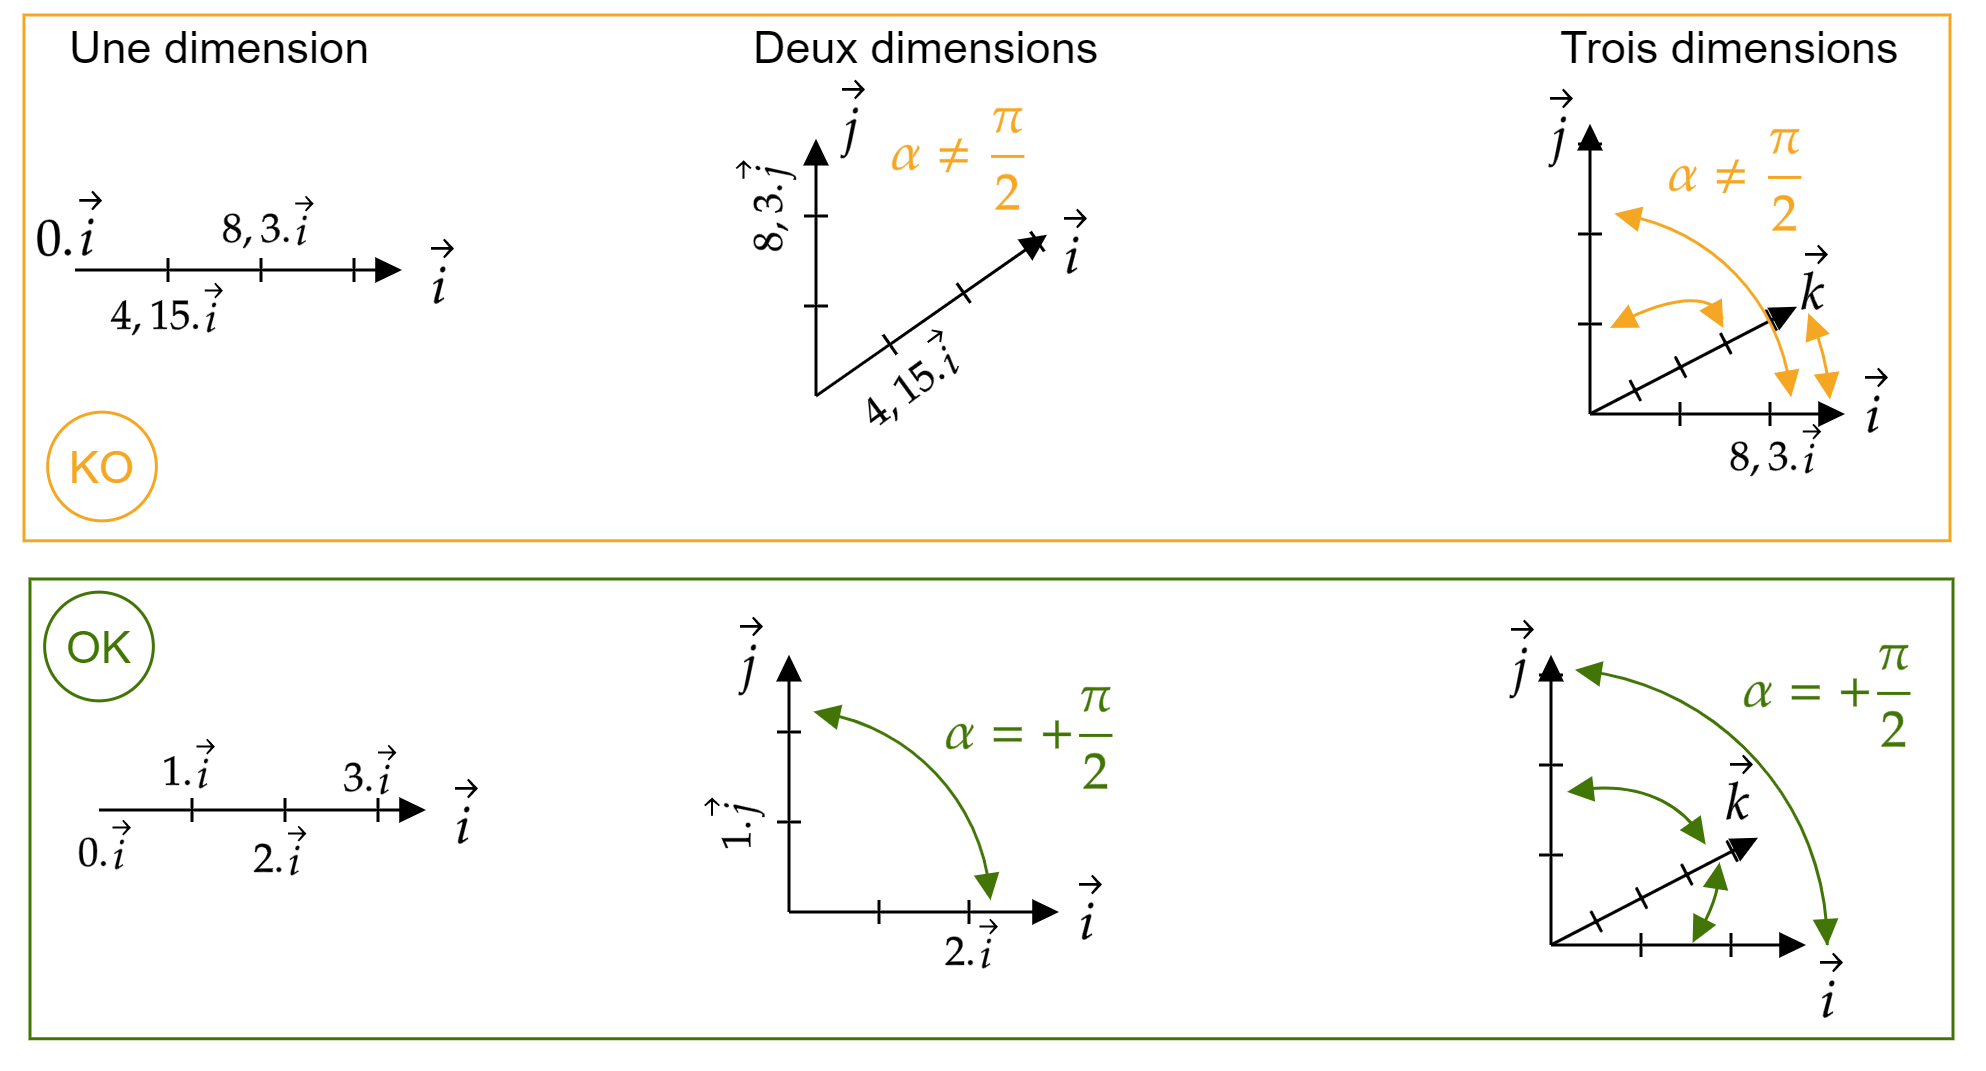
\includegraphics[width=1\textwidth]{Images/repere2.png} % Include the figure image
	\caption{Construction d'un repère pour dimension 1, 2 et 3.}
	\label{repere2} % Unique label used for referencing the figure in-text
\end{figure}


\begin{figure}[H] % Use [H] to suppress floating and place the figure/table exactly where it is specified in the text
	\centering % Horizontally center the figure on the page
	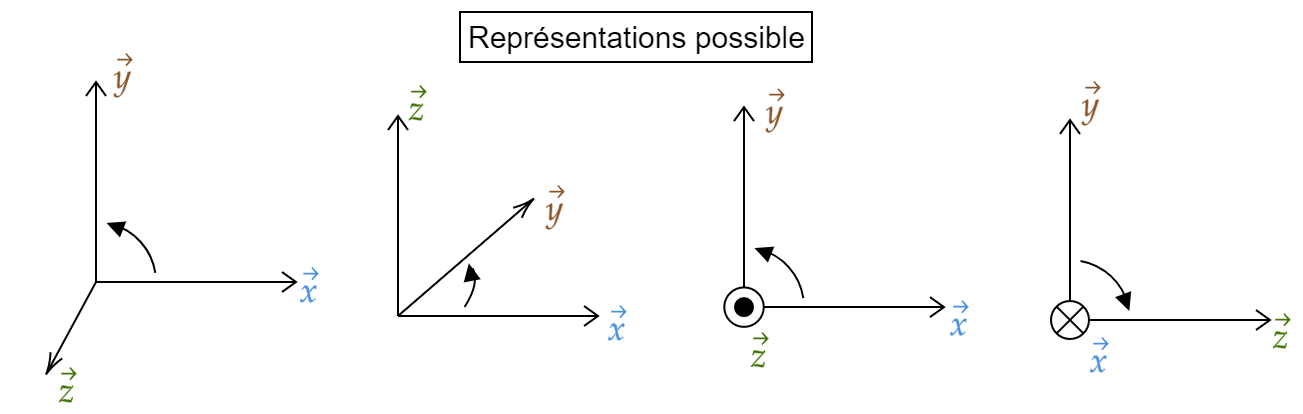
\includegraphics[width=1\textwidth]{Images/repere3.png} % Include the figure image
	\caption{Schémas type de repères en fonction du sens direct.}
	\label{repere3} % Unique label used for referencing the figure in-text
\end{figure}


Dans ses conditions on pourra utiliser les relations trigonométriques suivantes :

\vspace{0.5cm}
 

$\displaystyle \cos( \theta -\pi ) =\ -\cos( \theta )$ et $\displaystyle \sin( \theta +\pi ) =-\sin( \theta )$ \\

$\displaystyle \cos( \pi -\theta ) =-\cos( \theta )$ et $\displaystyle \sin( \pi -\theta ) =\sin( \theta )$ \\

$\displaystyle \cos( -\theta ) =\cos( \theta )$ et $\displaystyle \sin( -\theta ) =-\sin( \theta )$ \\

$\displaystyle \cos\left(\frac{\pi }{2} -\theta \right) =\sin( \theta )$ et $\displaystyle \sin\left(\frac{\pi }{2} -\theta \right) =\cos( \theta )$ \\

$\displaystyle \cos\left( \theta +\frac{\pi }{2}\right) =-\sin( \theta )$ et $\displaystyle \sin\left( \theta +\frac{\pi }{2}\right) =\cos( \theta )$ 

\section{Référentiel}
Un Référentiel , on ajoute $t$, le temps avec une unité (exemple : seconde), du labo, galiéen

\begin{figure}[H] % Use [H] to suppress floating and place the figure/table exactly where it is specified in the text
	\centering % Horizontally center the figure on the page
	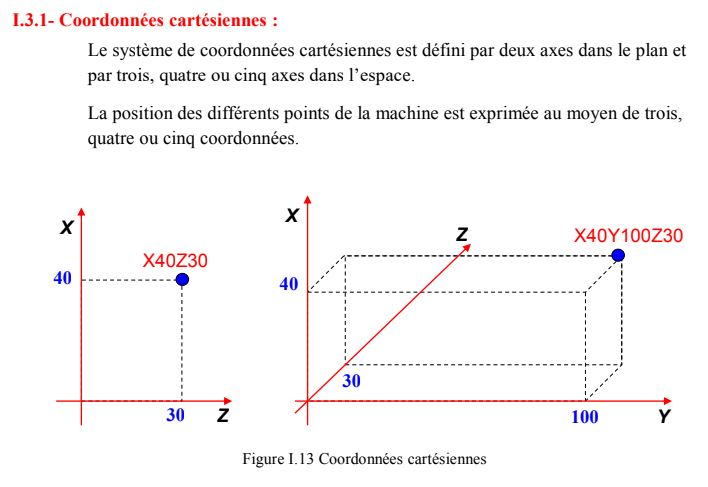
\includegraphics[width=1\textwidth]{Images/cart.JPG} % Include the figure image
	\caption{Logo de la certification QSE}
	\label{cart} % Unique label used for referencing the figure in-text
\end{figure}




\begin{figure}[H] % Use [H] to suppress floating and place the figure/table exactly where it is specified in the text
	\centering % Horizontally center the figure on the page
	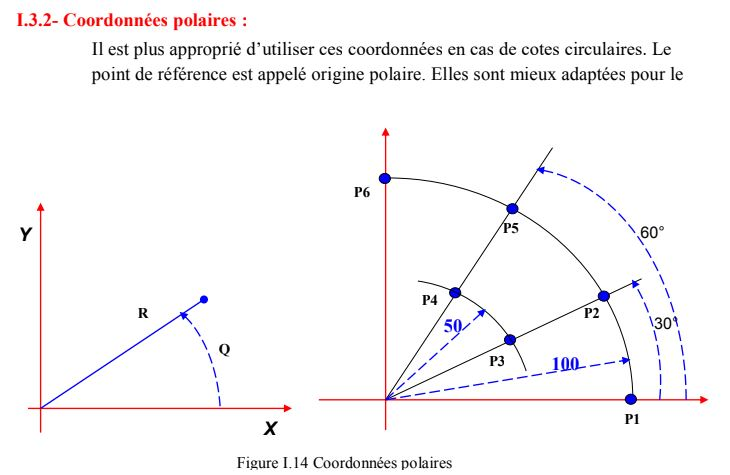
\includegraphics[width=1\textwidth]{Images/pol.JPG} % Include the figure image
	\caption{Le système de cordonnées (X, Y, Z) est un système cartésien de sens direct lié à une pièce placée sur la machine. Exemple : Sur une MOCN, on peut mettre manuellement en rotation la broche dans le sens direct en appuyant sur le bouton \textbf{C+} du pupitre de commande.}
	\label{pol4} % Unique label used for referencing the figure in-text
\end{figure}



%----------------------------------------------------------------------------------------
%	PRESENTING INFORMATION/RESULTS EXAMPLES CHAPTER
%----------------------------------------------------------------------------------------

\chapterimage{Images/chapt_F.jpg} % Chapter heading image
\chapterspaceabove{6.25cm} % Whitespace from the top of the page to the chapter title on chapter pages
\chapterspacebelow{7.5cm} % Amount of vertical whitespace from the top margin to the start of the text on chapter pages

%------------------------------------------------
\chapter{Représenter le réel}

\section{Introduction}









Pas parler de physique, rester math . un peu de math, vecteur exprime globalement tout avec une fleche ou un type de fleche (double fleche pour les moments)
\subsection{Notations}
vecteur (F ou M ou T ou V ou $\Vec{a}$ ou P), torseurs
\subsection{Vecteurs}\label{Vecteurs}

On écrivait comme ça,  $\Vec{i}=\ \begin{Bmatrix} a\\ b \\ c \end{Bmatrix} $  maintenant faut écrire comme ça 
 {$\mathcal{F}_{moteur} =\ \begin{Bmatrix}
F_{x}\\
F_{y}\\
F_{z}
\end{Bmatrix}_{( \mathcal{B}_{1} ,\ \vec{x} ,\ \vec{y} ,\vec{z})}$};

2D , 3D, certain sont constant $\overrightarrow{\mathcal{V}_{(train\rightarrow route)}} \ =\ C^{te}$ dautre nan $\overrightarrow{\mathcal{T}_{(train\rightarrow route)}} \ =\ X$ trajectoire



\subsection{Torseurs}
video science clic ?

\begin{Extrait}\index{Torseurs (exercice)}
TS CPRP 2015 \\
On se propose d’estimer l’effort maxi que doit appliquer la contre-pointe sur le papillon lors de l’opération de perçage. \\



\noindent \begin{minipage}{0.5\textwidth}
\vspace{1cm}
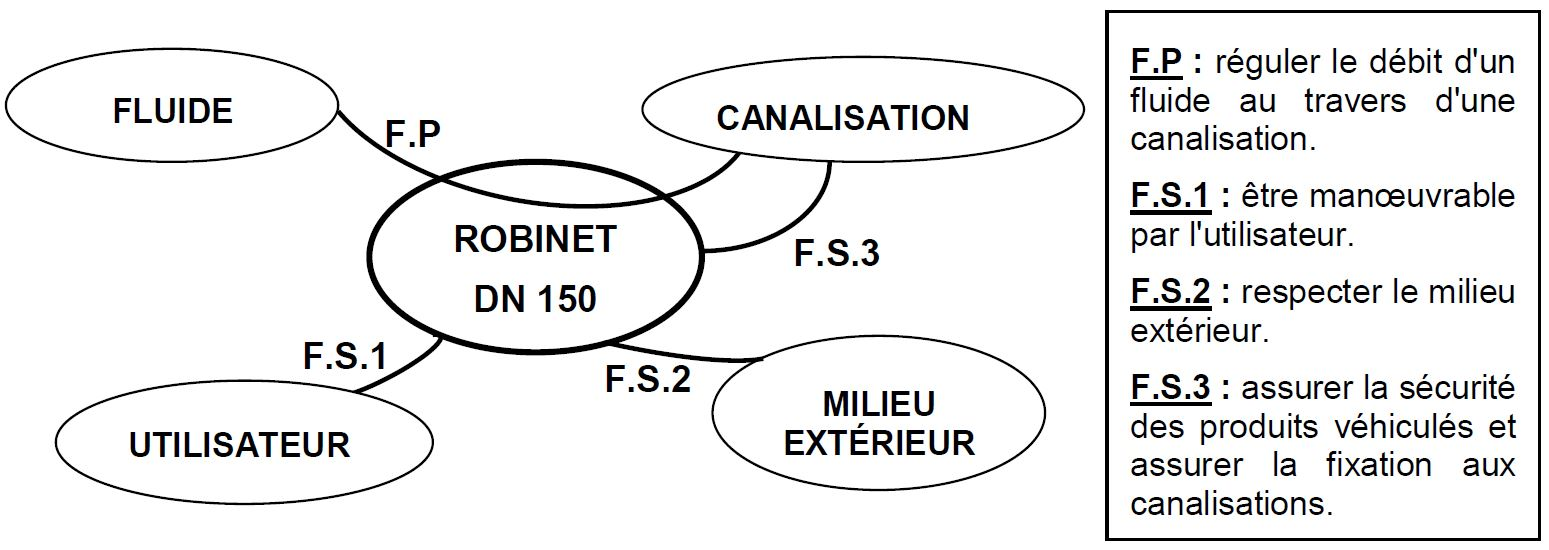
\includegraphics[width=1\textwidth]{Images/2015.JPG}
\label{fig:nature}
\end{minipage}
\hspace{0.05\textwidth}
\begin{minipage}{0.4\textwidth}
Hypothèses : 
\begin{itemize}
\item Le problème possède un plan de
symétrie mécanique ($\mathcal{B}, \Vec{y}, \Vec{z}$) ;
\item L’ensemble des contacts entre
solide se fait avec adhérence. On
prendra $tan(\phi_{0}) = 0,1.$ ;
\item L’étude est menée à la « limite du
glissement »;
\item L'action de la pesanteur est
négligée ;
\item Pour l’étude, l’effort de pénétration notée $\overrightarrow{\mathcal{A}_{(f\rightarrow p)}}\ $ aura une intensité de : \\ $ \Vert \overrightarrow{\mathcal{A}_{(f\rightarrow p)}} \Vert = 2000 N\ $
\end{itemize}

\end{minipage}


On notera :
$\displaystyle \begin{Bmatrix}
A_{f\rightarrow p}
\end{Bmatrix} =\begin{Bmatrix}
\overrightarrow{A_{f\rightarrow p}} =2000.\vec{y} & \\
\overrightarrow{\mathcal{M}_{A}{}_{\left( f\rightarrow p\right)}} =\vec{0} & 
\end{Bmatrix}_{A,\ (\mathcal{R} ,\ \vec{x} ,\ \vec{y} ,\ \vec{z})}$

Concernant l’action de posage, on considère que la liaison entre les supports à bille
oscillante et le papillon est une liaison appui plan. En l’absence de mouvement, le
torseur modélisant l’action mécanique transmissible comporte 3 inconnues Yc, Zc et Lc.
Comme la liaison est unilatérale, ZC > 0.

$\displaystyle \begin{Bmatrix}
C_{pp\rightarrow papillon}
\end{Bmatrix} =\begin{Bmatrix}
0 & L_{c}\\
Y_{c} & 0\\
Z_{c} & 0
\end{Bmatrix}_{C,\ (\mathcal{R} ,\ \vec{x} ,\ \vec{y} ,\ \vec{z})} avec\ Y_{c} =Z_{c} .\tan( \phi_{0})$


\end{Extrait}




\section{Position, vitesse et accélération}
Mettre le sens physique
\subsection{Vecteur trajectoire}

\section{Forces}

\section{Moments / Couples}

\section{Notations}

\begin{definition}\index{Solide indéformable}
Un solide indéformable $\mathcal{S}$ est caractérisé par un ensemble de points, la distance entre deux points étant invariante au cours du temps. \\


    $ \forall \ t,\forall A\ \in S,\ \forall B\ \in S\ :\ \Vert \overrightarrow{AB}\Vert =C^{cte} \ $ 


\textit{On lit la ligne du dessus comme suit :} Quelque chose est un solide si, pour tout instant $t$, pour tous points $A$ d'un solide $\mathcal{S}$, pour tout point $B$ appartenant aussi à $\mathcal{S}$, la distance entre les points $A$ et $B$ reste constant au cours du temps.
    
\end{definition}


\begin{corollary}[S2.4] 
aze
\end{corollary}

\begin{definition}{Normes}\index{Norme}
aze
\end{definition}

\begin{theorem}
    sqdf
\end{theorem}

\begin{remark}
    aze
\end{remark}






%----------------------------------------------------------------------------------------
%	PRESENTING INFORMATION/RESULTS EXAMPLES CHAPTER
%----------------------------------------------------------------------------------------

\chapterimage{Images/A6.jpg} % Chapter heading image
\chapterspaceabove{6.25cm} % Whitespace from the top of the page to the chapter title on chapter pages
\chapterspacebelow{7.5cm} % Amount of vertical whitespace from the top margin to the start of the text on chapter pages

%------------------------------------------------


	




\newpage
\section{ANNEXE}


\phantomsection
\addcontentsline{toc}{chapter}{\textcolor{ocre}{Index}} % Add an Index heading to the table of contents
\printindex % Output the index


\end{document}


